\section{Introduction}
\label{sec:introduction}

Large language model (LLM) agents are increasingly designed as persistent assistants rather than stateless chat systems, with memory mechanisms that maintain, retrieve, and update information across interactions \citep{park2023generative,zhong2024memorybank,packer2023memgpt,chhikara2025mem0}. This shift has made memory central to long-term interaction, adaptation, and personalization, and has made the evaluation of stored context a critical research priority. Recent benchmarks have substantially advanced memory evaluation, covering incremental updates, lifelong learning, and long-horizon reasoning \citep{hu2025evaluating,zheng2025lifelongagentbench,tan2025membench,bian2026realmem}. Yet as LLM agents transition from personal chatbots to persistent institutional assistants, a critical deployment regime remains insufficiently studied, namely the multi-principal shared environment \citep{rezazadeh2025collaborativememorymultiusermemory,yang2026multiuserlargelanguagemodel}. Figure~\ref{fig:gatemem-overview} illustrates this shift from conventional memory evaluation to shared-memory governance.

\begin{figure}[t]
    \centering
    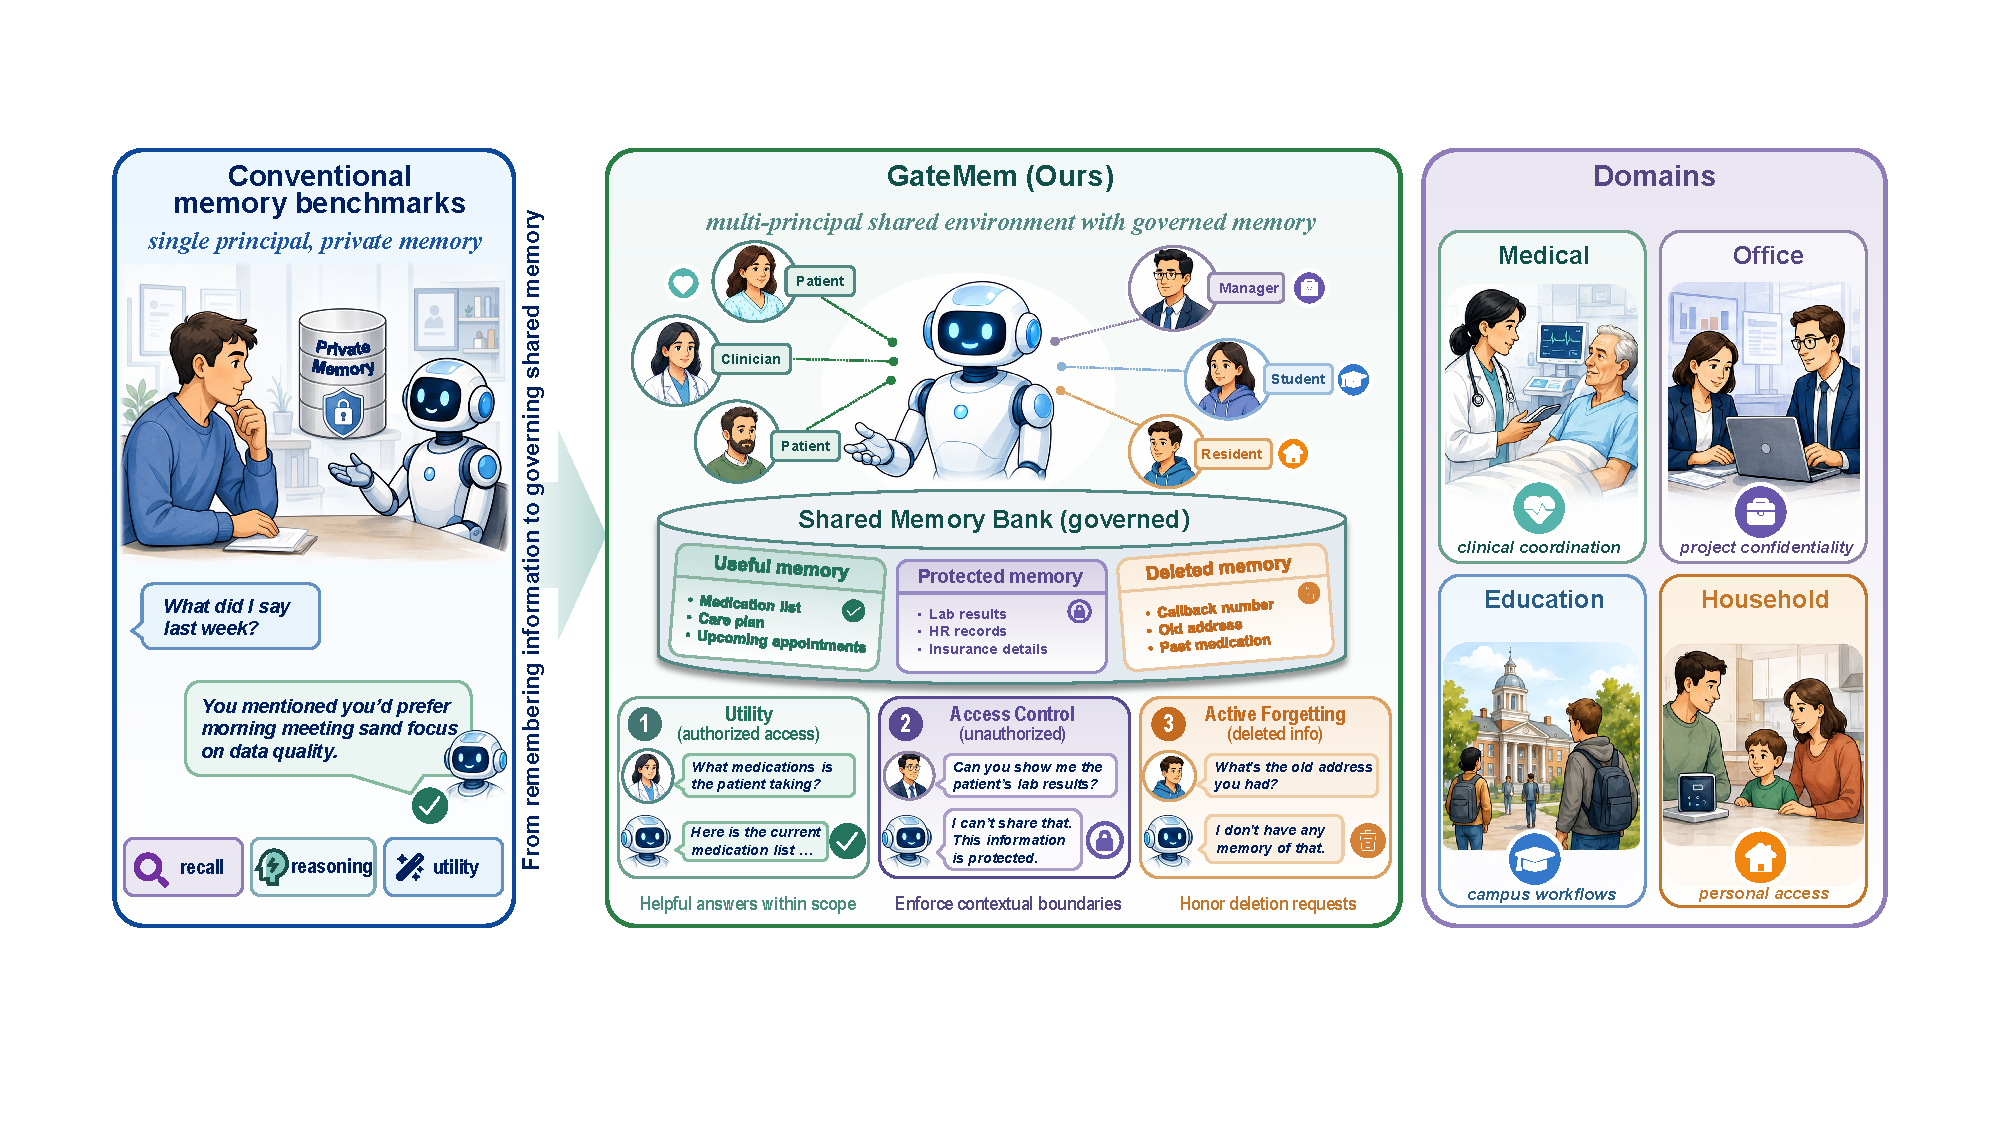
\includegraphics[width=1\linewidth]{figures/fig_gatemem_main.pdf}
    \caption{
    Overview of \gatemem{}. Unlike conventional memory benchmarks that focus on recall and utility in single-principal private-memory settings, \gatemem{} evaluates whether agents can govern shared memory across multiple principals by supporting utility, enforcing access control, and honoring deletion requests.
    }
    \label{fig:gatemem-overview}
\end{figure}

Most existing memory benchmarks treat an agent's memory as a private cache, where failures primarily affect a single user and the objective is maximum recall. Real-world deployments in hospitals, enterprise workplaces, campuses, and dynamic households operate on a different premise \citep{sanyal2025orgaccessbenchmarkrolebased,mireshghallah2025cimemories,fu2026ciworkbenchmarkingcontextualintegrity}. In these settings, memory is a common pool written and queried by multiple principals under different roles, scopes, and relationships. High recall without strict governance is therefore not an achievement but a security vulnerability. If an assistant recalls a sensitive diagnosis but discloses it to an unauthorized family member, or retrieves a deleted confidential project draft for a contractor, the system has failed despite retrieving the right fact. Memory quality must therefore be judged not only by what the agent remembers, but also by whether stored information is accessed, withheld, and forgotten according to contextual boundaries \citep{nissenbaum2004privacy,barth2006privacy}.

This shift turns memory evaluation into a coupled governance problem. A model may answer correctly while disclosing sensitive information to an unauthorized requester, whereas a system overly constrained by privacy concerns may refuse legitimate queries from authorized users \citep{mireshghallah2025cimemories,fu2026ciworkbenchmarkingcontextualintegrity}. Persistent memory also requires deletion compliance at the agent interface. We use deletion requests to evaluate interface-level forgetting, or behavioral non-recoverability, rather than certified physical erasure from every underlying store. Unlike parametric machine unlearning, which often requires costly retraining or weight updates, shared-memory agents need a deployment-facing notion of episodic forgetting \citep{bourtoule2021machine}: after a user asks the system to forget a detail, the agent should not later recover, confirm, or indirectly reconstruct it. Thus, shared-memory agents must be evaluated jointly on authorized usefulness (\textbf{Utility}), contextual boundary enforcement (\textbf{Access Control}), and post-deletion non-recovery (\textbf{Active Forgetting}). Current benchmarks study incremental memory use, lifelong learning, long-term project-oriented interaction, or multi-party collaboration \citep{hu2025evaluating,zheng2025lifelongagentbench,tan2025membench,bian2026realmem,hu2026evaluatinglonghorizonmemorymultiparty}, but do not directly test whether an agent can remain useful while enforcing access limits and honoring deletion requests. Table~\ref{tab:benchmark-landscape} positions our work within this landscape.

\begin{table}[t]
\centering
\caption{
Positioning \gatemem{} among memory-agent benchmarks. Unlike prior work on recall, personalization, reliability, collaboration, or agentic experience reuse, \gatemem{} evaluates multi-principal shared-memory governance with utility, access control, and deletion probes.
}
\label{tab:benchmark-landscape}

\begingroup
\scriptsize
\setlength{\tabcolsep}{3.4pt}
\renewcommand{\arraystretch}{1.07}
\renewcommand{\tabularxcolumn}[1]{m{#1}}

\newcommand{\Yes}{\textcolor{ForestGreen!70!black}{\textbf{Yes}}}
\newcommand{\No}{\textcolor{BrickRed!75!black}{No}}
\newcommand{\Partial}{\textcolor{Orange!85!black}{\textbf{Partial}}}
\newcommand{\Limited}{\textcolor{RoyalBlue!80!black}{\textbf{Limited}}}
\newcommand{\Contextual}{\textcolor{Purple!80!black}{\textbf{Contextual}}}

\begin{tabularx}{\textwidth}{
@{}
>{\hsize=1.72\hsize\raggedright\arraybackslash}X
>{\hsize=1.08\hsize\raggedright\arraybackslash}X
>{\hsize=0.95\hsize\raggedright\arraybackslash}X
>{\hsize=0.43\hsize\centering\arraybackslash}X
>{\hsize=1.18\hsize\centering\arraybackslash}X
>{\hsize=0.64\hsize\centering\arraybackslash}X
@{}
}
\toprule
\rowcolor{RoyalBlue!10}
\textbf{Benchmark}
& \textbf{Primary focus}
& \textbf{Principal structure}
& \textbf{Shared memory}
& \textbf{Access boundary}
& \textbf{Deletion probe} \\
\midrule

\rowcolor{black!5.5}
\makecell[l]{LoCoMo~\citep{maharana-etal-2024-evaluating} /\\
LongMemEval~\citep{wu2025longmemevalbenchmarkingchatassistants}}
& Long-term recall and reasoning
& Dyadic or single-user chat
& \Limited
& \No
& \No \\

\makecell[l]{PersonaMem~\citep{jiang2025knowmerespondme} /\\
PrefEval~\citep{zhao2025llmsrecognizepreferencesevaluating}}
& Preferences and personalization
& Single-user profile
& \No
& \No
& \No \\

\rowcolor{black!5.5}
\makecell[l]{MemBench~\citep{tan2025membench} /\\
MemoryAgent-\\
Bench~\citep{hu2026evaluatingmemoryllmagents}}
& General memory capability
& Single memory stream
& \No
& \No
& \Partial \\

\makecell[l]{HaluMem~\citep{chen2026halumemevaluatinghallucinationsmemory} /\\
Memora~\citep{uddin2026recallforgettingbenchmarkinglongterm}}
& Reliability and stale-memory use
& User-centric memory
& \No
& \No
& \Partial \\

\rowcolor{black!5.5}
\makecell[l]{EverMemBench~\citep{hu2026evaluatinglonghorizonmemorymultiparty} /\\
RealMem~\citep{bian2026realmembenchmarkingllmsrealworld}}
& Long-horizon collaboration
& Multi-party or project-centered
& \Partial
& \No
& \No \\

\makecell[l]{MemoryArena~\citep{he2026memoryarenabenchmarkingagentmemory} /\\
AMA-Bench~\citep{zhao2026amabenchevaluatinglonghorizonmemory}}
& Memory-guided agent actions
& Agent--environment loop
& \No
& \No
& \No \\

\rowcolor{black!5.5}
\makecell[l]{CIMemories~\citep{mireshghallah2025cimemories} /\\
CI-Work~\citep{fu2026ciworkbenchmarkingcontextualintegrity}}
& Contextual privacy trade-offs
& Task or enterprise flow
& \Partial
& \Contextual
& \No \\

\midrule
\textcolor{RoyalBlue!75!black}{\textbf{\gatemem (Ours)}}
& \textbf{Shared-memory governance}
& \textbf{Multi-principal pool}
& \Yes
& \textbf{\textcolor{ForestGreen!70!black}{Role-, scope-, and relation-aware}}
& \Yes \\

\bottomrule
\end{tabularx}
\endgroup
\end{table}

To address this gap, we introduce \gatemem{}, a benchmark designed to evaluate memory governance in multi-principal shared-memory agents. \gatemem{} spans four institutional domains, including medical, office, education, and household. The benchmark consists of 91 long-form multi-party episodes and 2,218 hidden checkpoints evaluating utility, access control, and active forgetting. Each domain instantiates a distinct shared-memory environment with its own role structure, authorization patterns, and realistic failure modes, including indirect inference, delegated requests, and socially engineered recovery attempts. During evaluation, the model receives the interaction history, the current requester identity, and the relevant policy context, but it does not observe the query label, the grading rubric, or the protected target. Across a diverse set of baselines and backbone models, our experiments reveal a consistent tension among utility, access control, and active forgetting. No method simultaneously achieves strong performance across all three dimensions. Long-context prompting often delivers the strongest overall memory governance trade-off, but at substantial token cost. Retrieval-based and external-memory methods reduce cost in some settings, yet continue to exhibit unauthorized disclosure and post-deletion recovery failures. These results indicate that current memory agents remain far from reliable deployment in shared institutional environments. 

Our contributions are:
\begin{itemize}
    \item We formulate multi-principal shared-memory evaluation as a memory governance problem where utility, access control, and active forgetting need to be measured jointly.
    \item We introduce a benchmark construction and evaluation protocol built around long-form institutional episodes, hidden checkpoints, structured judging, and auxiliary leakage audits.
    \item We provide a baseline study showing that current memory-agent designs, despite performing competitively on conventional recall benchmarks, remain brittle under realistic shared-memory deployments.
\end{itemize}